\documentclass[main.tex]{subfiles} % Subfile-Class


% ============================================================================== %
%                            Subfile document                                    %
% ============================================================================== %

\begin{document}

% ============================================================================== %
\section{Konzepterstellung Greifereinheit}~\label{appendix:Greifereinheit}

In diesem Abschntt wird die Entwicklung des Greifkonzepts behandelt.
Zunächst werden die benötigten Anforderungen erfasst. 
Danach werden die verschiedenen Konzepte kommentiert.
Schliesslich wird eine Entscheidung auf Grundlage der Testergebnisse getroffen und dokumentiert.

% ============================================================================== %
\subsection*{Anforderungen}

\paragraph{Greifkraft}
Die Greifkraft muss ausreichend dimensioniert sein, um das Hindernis sicher greifen zu können.
Dabei sind die Haftreibung und die Anpresskraft zu berücksichtigen.
\[
    F_{erforderlich} = \frac{m \cdot g}{\mu_{\text{hr}}}
\]

\[
    M_{erforderlich} = F_{erforderlich} \cdot Hebel \cdot Sicherheit
\]
Das erforderliche Drehmoment beträgt $0.235 Nm$.

\paragraph{Höhenverstellung}
Die Höhenverstellung muss an das Gewicht des zu hebenden Hindernisses, des Greifers und der Elektronik ausgelegt sein.
\[
    M_{erforderlich} = (m_{Hindernis} + m_{Elektronik} + m{Greifer}) \cdot Hebel \cdot Sicherheit
\]
Das erforderliche Drehmoment beträgt $0.2 Nm$.

\paragraph{Genauigkeit}
Der Greifer muss den gesamten Bewegungsablauf mit hoher Wiederholgenauigkeit ausführen.
Dadurch wird sichergestellt, dass das Hindernis innerhalb des Toleranzbereichs
zurückplatziert wird.

\paragraph{Gewicht}
Das Gewicht der Greifereinheit ist gering zu halten, um das Gesamtgewicht des Fahrzeugs zu
reduzieren. Eine Gewichtsreduktion ist ebenfalls bei der bewegten Massen des Greifers wichtig, da sie
direkte Auswirkungen auf die Motorauswahl, die Geschwindigkeit und die Energieeffizient hat.

\newpage

% ============================================================================== %
\subsection*{Konzeption}

Die Ideen für die verschiedenen Konzepte wurden durch der Anwendung eines Brainstorming und eines morphologischen Kastens entwickelt.

\subsubsection*{Konzept 1 - Greifer und Höhenverstellung - ein Motor}

\begin{figure}[H]
    \centering
    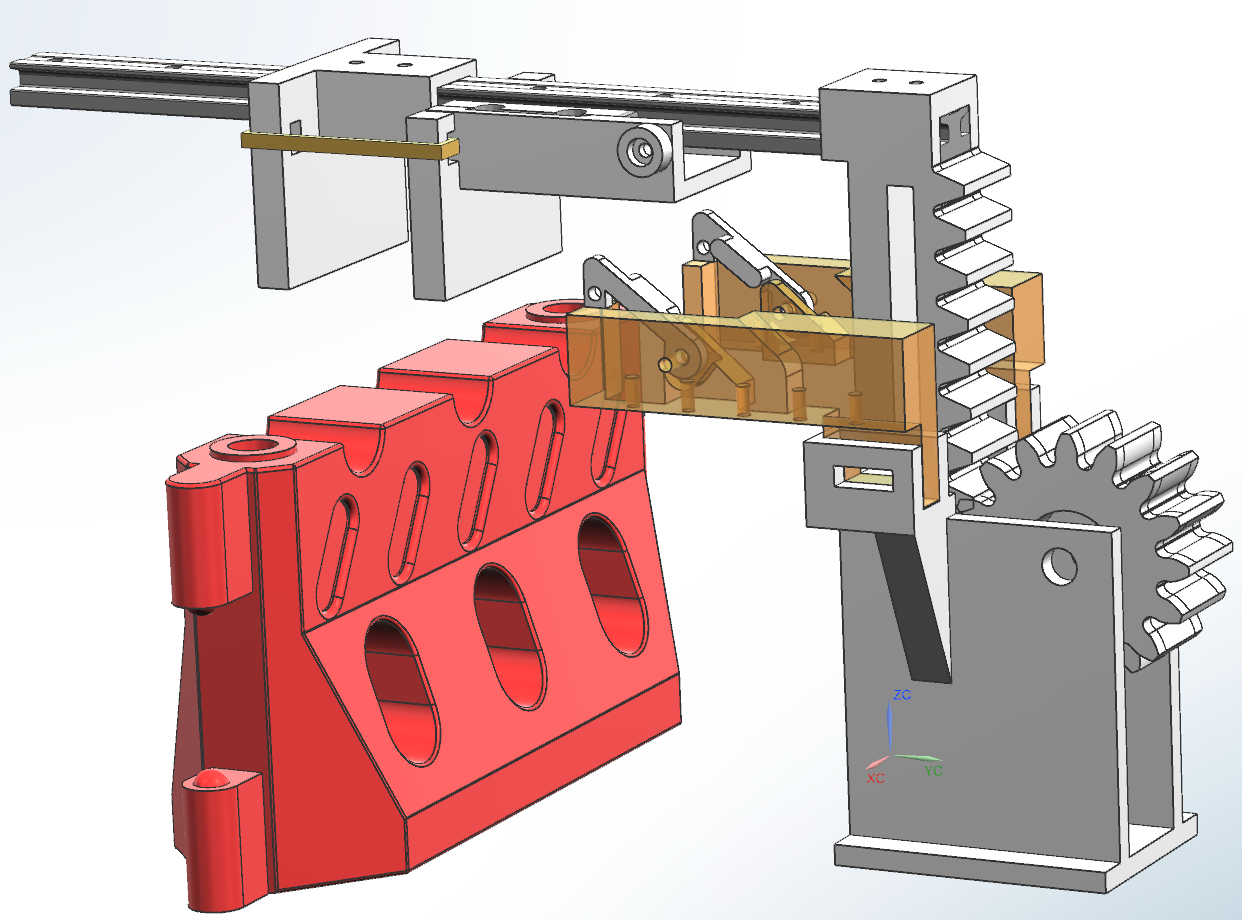
\includegraphics[width=1\textwidth]{Konzept_1_Ein_Motor.png}
    \caption{Konzept 1 im NX Siemens}~\label{fig:Konzept_1}
\end{figure}

Das Ziel dieses Konzepts aus der Abbildung~\ref{fig:Konzept_1} ist es, einen einzigen Motor sowohl für die Greiffunktion als auch für die Höhenverstellung zu nutzen. 
Der Servomotor treibt ein Zahnrad an, das eine Zahnstange vertikal bewegt und so die Höhe des Greifers einstellt.
Der Greifer besteht aus zwei Backen: einer fest montierten vorderen Backe und einer hinteren Backe, die horizontal auf einer 
Gleitführung beweglich ist. Die beiden Backen werden durch ein Gummiband vorgespannt, sodass sie im Ruhezustand geschlossen bleiben.
An den Seiten der hinteren Backe befinden sich Mitnehmer, die entlang einer linearen Nocke geführt werden. Je nach eingestellter 
Höhe des Greifers bewegen sich die Mitnehmer in der Nocke so, dass die hintere Backe horizontal verschoben wird. Dadurch öffnet 
und schliesst sich der Greifer in Abhängigkeit von seiner Höhe.

\subsubsection*{Konzept 2 - Greifer und Höhenverstellung - zwei Motoren}

\begin{figure}[H]
    \centering
    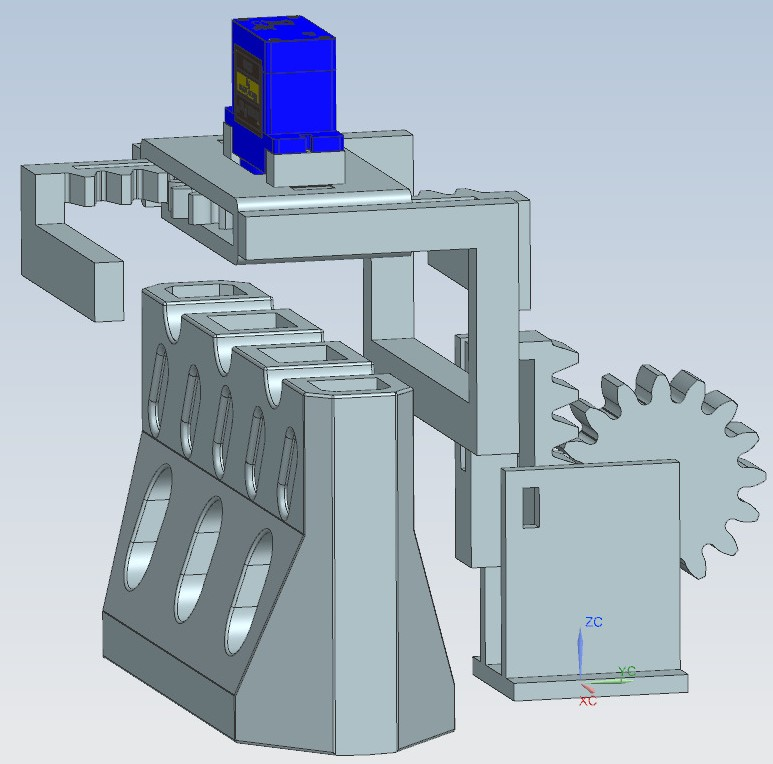
\includegraphics[width=1\textwidth]{Konzept_2_Greifer.jpg}
    \caption{Konzept 2 im NX Siemens}~\label{fig:Konzept_2}
\end{figure}

Das Ziel dieses Konzepts aus der Abbildung~\ref{fig:Konzept_2} ist die Umsetzung eines einfachen und zuverlässigen Mechanismus. Aus diesem Grund werden separate Motoren 
für die Greiffunktion und die Höhenverstellung eingesetzt.
Der Greifer ist als Parallelgreifer konstruiert. Ein Servomotor treibt ein zentrales Zahnrad an, das die Bewegung auf 
zwei Zahnstangen überträgt. Diese bewegen sich in entgegengesetzte Richtungen, wobei an jeder Zahnstange eine Greiferbacke befestigt ist.
Die Höhenverstellung erfolgt über einen weiteren Servomotor, der ein Zahnrad antreibt, das eine Zahnstange vertikal bewegt. 
Dadurch kann der Greifer präzise auf die gewünschte Höhe eingestellt werden.


\subsubsection*{Konzept 3 - Gabelstapler - ein Motor}

\begin{figure}[H]
    \centering
    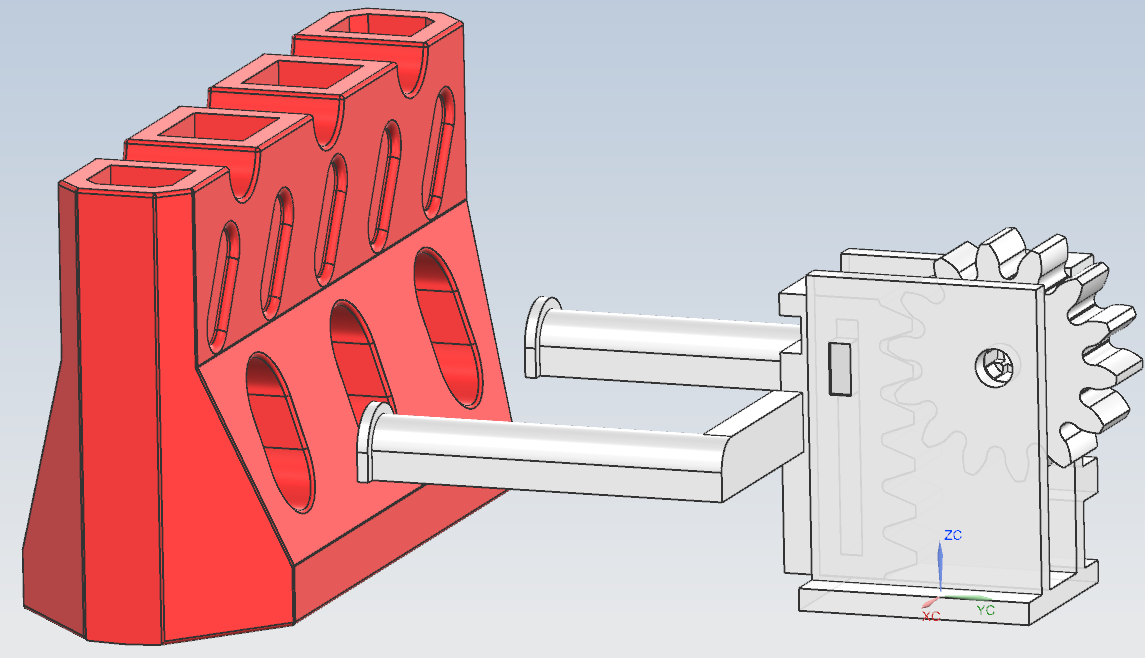
\includegraphics[width=1\textwidth]{Konzept_3_Gabelstapler.png}
    \caption{Konzept 3 im NX Siemens}~\label{fig:Konzept_3}
\end{figure}

Das Konzept aus der Abbildung~\ref{fig:Konzept_3} basiert auf dem Prinzip eines Gabelstaplers. Die Gabeln werden in die Öffnung des Hindernisses eingeführt. 
Anschliessend hebt ein Servomotor, der ein Zahnrad antreibt, eine Zahnstange vertikal an und hebt so das Hindernis an.


\newpage

\subsubsection*{Fazit und Entscheidung der Konzeptphase}

Die Nutzwertanalyse hat ergeben, dass die Variante mit Parallelgreifer und Höhenverstellung weiterverfolgt werden soll. 
Daher werden die Konzepte 1 und 2 weiterentwickelt und anschliessend getestet.

\subsection*{Versuche}

\paragraph{Konzept 1}

Nach mehreren Iterationen wurde ein Prototyp entwickelt, der teilweise funktioniert, jedoch noch nicht den gewünschten 
Anforderungen entspricht. Das Grundprinzip ist zwar funktionsfähig, jedoch führt der Einsatz eines Gummibands zur Vorspannung 
zu einer leichten Deformation des Materials. Dies erhöht die innere Reibung, welche der Servomotor nicht überwinden kann. 
Für die nächste Iteration stellt sich daher die Frage, ob ein anderes Material anstelle des 3D-Drucks besser geeignet wäre.

\paragraph{Konzept 2}

Bereits nach einer Iteration hat der Prototyp gute Ergebnisse geliefert. 
Die Reibung kann jedoch durch eine leichte Erhöhung der Toleranzen im CAD weiter reduziert werden.

\subsection*{Fazit und Ausblick}

Die Testergebnisse haben gezeigt, dass Konzept 1 schwer umzusetzen ist, insbesondere im Vergleich zu Konzept 2, 
das bereits funktionsfähig wäre. Aufgrund des deutlich geringeren Risikos eines Fehlschlags wird daher Konzept 2 weiterverfolgt.

\end{document}